\section{Introduction}
\label{sec:intro}

In the past few years, there has been an explosion of interest in LLMs with the creation of widely available resources like OpenAI's ChatGPT
and Meta's open source Llama. Much of the explosion has been driven by the creation of the transformer architecture, which has made a dramatic difference throughout AI, but particularly in the world of LLMs. However, our fundamental understanding of how these objects remains shrouded in mystery.

Because of our lack of understanding of how these objects work, and the quick assimilation of these products into our daily lives, there are a variety of novel security risks that we are being introduced to. One specific error is not so common, but still of practical relevance, is a hardware failure in which a random bitflip occurs in the parameters of our model. An error of such a fashion could have drastic effects on our output, ranging from making the outputs gibberish to outright wrong.

In this paper, we analyze how injecting bit errors into specific locations of a transformer and the LLM model as a whole affect the output. To this end, we use the GPT2 as a base model to test on. To inject errors into our base model we use the PyTEI package \cite{Ma23}. To quantify the effect of our errors, we compare the score of our base model to the score of the models with errors injected using the PyTEI package with DeepEval to evaluate.


Our basic workflow is outlined in the below diagram

\begin{figure}[ht]
	\begin{center}
		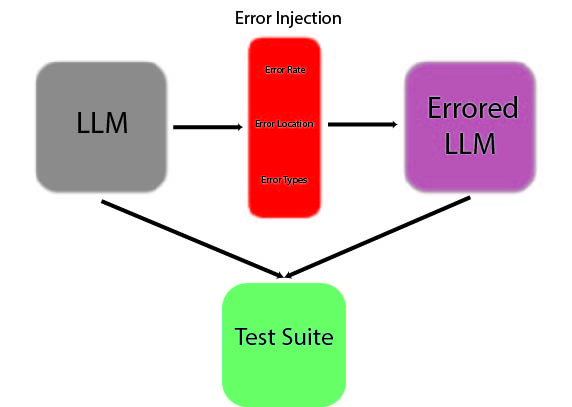
\includegraphics[height=6cm]{workflow.jpg}
		\caption{General evaluation workflow for LLM}
		\label{workflow}
	\end{center}
\end{figure}





%%% Local Variables:
%%% mode: latex
%%% TeX-master: "main"
%%% End:

%  LocalWords:  biometrics cryptographic parallelized lossy
